\section{予測符号化}
\subsection{観測世界の階層的予測}
\textbf{階層的予測符号化(hierarchical predictive coding; HPC)}\index{かいそうてきよそくふごうか(hierarchical predictive coding; HPC)@階層的予測符号化(hierarchical predictive coding; HPC)} は\citep{Rao1999-zv}により導入された.構築するネットワークは入力層を含め,3層のネットワークとする.LGNへの入力として画像 $\mathbf{x} \in \mathbb{R}^{n_0}$を考える.画像 $\mathbf{x}$ の観測世界における隠れ変数,すなわち\textbf{潜在変数}\index{せんざいへんすう@潜在変数} (latent variable)を$\mathbf{r} \in \mathbb{R}^{n_1}$とし,ニューロン群によって発火率で表現されているとする (真の変数と $\mathbf{r}$は異なるので文字を分けるべきだが簡単のためにこう表す).このとき,
\begin{equation}
\mathbf{x} = f(\mathbf{U}\mathbf{r}) + \boldsymbol{\epsilon}
\end{equation}
が成立しているとする.ただし,$f(\cdot)$は活性化関数 (activation function),$\mathbf{U} \in \mathbb{R}^{n_0 \times n_1}$は重み行列である.$\boldsymbol{\epsilon} \in \mathbb{R}^{n_0}$ は $\mathcal{N}(\mathbf{0}, \sigma^2 \mathbf{I})$ からサンプリングされるとする.潜在変数 $\mathbf{r}$はさらに高次 (higher-level)の潜在変数 $\mathbf{r}^h$により,次式で表現される.
\begin{equation}
\mathbf{r} = \mathbf{r}^{td}+\boldsymbol{\epsilon}^{td}=f(\mathbf{U}^h \mathbf{r}^h)+\boldsymbol{\epsilon}^{td}
\end{equation}
ただし,Top-downの予測信号を $\mathbf{r}^{td}\triangleqf(\mathbf{U}^h \mathbf{r}^h)$ とした.また,$\mathbf{r}^{td} \in \mathbb{R}^{n_1}$, $\mathbf{r}^{h} \in \mathbb{R}^{n_2}$, $\mathbf{U}^h \in \mathbb{R}^{n_1 \times n_2}$ である.$\boldsymbol{\epsilon}^{td} \in \mathbb{R}^{n_1}$は$\mathcal{N}(\mathbf{0}$, $\sigma_{td}^2 \mathbf{I}$) からサンプリングされるとする.
話は飛ぶが,Predictive codingのネットワークの特徴は
\begin{itemize}
\item 階層的な構造
\item 高次による低次の予測 (Feedback or Top-down信号)
\item 低次から高次への誤差信号の伝搬 (Feedforward or Bottom-up 信号)
\end{itemize}
である.ここまでは高次表現による低次表現の予測,というFeedback信号について説明してきたが,この部分はSparse codingでも同じである.それではPredictive codingのもう一つの要となる,低次から高次への予測誤差の伝搬というFeedforward信号はどのように導かれるのだろうか.結論から言えば,これは復元誤差 (reconstruction error)の最小化を行う再帰的ネットワーク (recurrent network)を考慮することで自然に導かれる.
\subsection{損失関数と学習則}
\subsubsection{事前分布の設定}
$\mathbf{r}$の事前分布$p(\mathbf{r})$はCauchy分布を用いる.$p(\mathbf{r})$の負の対数事前分布を$g(\mathbf{r})\triangleq-\log p(\mathbf{r})$としておく.
\begin{align}
p(\mathbf{r})&=\prod_i p(r_i)=\prod_i \exp\left[-\alpha \ln(1+r_i^2)\right]\\
g(\mathbf{r})&=-\ln p(\mathbf{r})=\alpha \sum_i \ln(1+r_i^2)\\
g'(\mathbf{r})&=\frac{\partial g(\mathbf{r})}{\partial \mathbf{r}}=\left[\frac{2\alpha r_i}{1+r_i^2}\right]_i
\end{align}
次に重み行列$\mathbf{U}$の事前分布 $p(\mathbf{U})$はGaussian分布とする.$p(\mathbf{U})$の負の対数事前分布を$h(\mathbf{U})\triangleq-\ln p(\mathbf{U})$とすると,次のように表される.
\begin{align}
p(\mathbf{U})&=\exp(-\lambda\|\mathbf{U}\|^2_F)\\
h(\mathbf{U})&=-\ln p(\mathbf{U})=\lambda\|\mathbf{U}\|^2_F\\
h'(\mathbf{U})&=\frac{\partial h(\mathbf{U})}{\partial \mathbf{U}}=2\lambda \mathbf{U}
\end{align}
ただし,$\|\cdot \| _ F^2$はフロベニウスノルムを意味する.
\subsubsection{損失関数の設定}
Sparse codingと同様に考えることにより,損失関数 $E$を次のように定義する.
\begin{align}
E=\underbrace{\frac{1}{\sigma^{2}}\|\mathbf{x}-f(\mathbf{U} \mathbf{r})\|^2+\frac{1}{\sigma_{t d}^{2}}\left\|\mathbf{r}-f(\mathbf{U}^h \mathbf{r}^h)\right\|^2}_{\text{reconstruction error}}+\underbrace{g(\mathbf{r})+g(\mathbf{r}^{h})+h(\mathbf{U})+h(\mathbf{U}^h)}_{\text{sparsity penalty}}
\end{align}
潜在変数 $\mathbf{r}, \mathbf{r}^h$ と 重み行列 $\mathbf{U}, \mathbf{U}^h$ のそれぞれに事前分布を仮定しているため,これらについてのMAP推定を行うことに相当する.
\subsubsection{再帰ネットワークの更新則}
簡単のために$\mathbf{z}\triangleq\mathbf{U}\mathbf{r}, \mathbf{z}^h\triangleq\mathbf{U}^h\mathbf{r}^h$とする.
\begin{align}
\frac{d \mathbf{r}}{d t}&=-\frac{k_{1}}{2} \frac{\partial E}{\partial \mathbf{r}}=k_{1}\cdot\Bigg(\frac{1}{\sigma^{2}} \mathbf{U}^{T}\bigg[\frac{\partial f(\mathbf{z})}{\partial \mathbf{z}}\odot\underbrace{(\mathbf{x}-f(\mathbf{z}))}_{\text{bottom-up error}}\bigg]-\frac{1}{\sigma_{t d}^{2}}\underbrace{\left(\mathbf{r}-f(\mathbf{z}^h)\right)}_{\text{top-down error}}-\frac{1}{2}g'(\mathbf{r})\Bigg)\\
\frac{d \mathbf{r}^h}{d t}&=-\frac{k_{1}}{2} \frac{\partial E}{\partial \mathbf{r}^h}=k_{1}\cdot\Bigg(\frac{1}{\sigma_{t d}^{2}}(\mathbf{U}^h)^\top\bigg[\frac{\partial f(\mathbf{z}^h)}{\partial \mathbf{z}^h}\odot\underbrace{\left(\mathbf{r}-f(\mathbf{z}^h)\right)}_{\text{bottom-up error}}\bigg]-\frac{1}{2}g'(\mathbf{r}^h)\Bigg)
\end{align}
ただし,$k_1$は更新率 (updating rate)である.または,発火率の時定数を$\tau\triangleq1/k_1$として,$k_1$は発火率の時定数$\tau$の逆数であると捉えることもできる.ここで1番目の式において,中間表現 $\mathbf{r}$ のダイナミクスはbottom-up errorとtop-down errorで記述されている.このようにbottom-up errorが $\mathbf{r}$ への入力となることは自然に導出される.なお,top-down errorに関しては高次からの予測 (prediction)の項 $f(\mathbf{x}^h)$とleaky-integratorとしての項 $-\mathbf{r}$に分割することができる.また$\mathbf{U}^\top, (\mathbf{U}^h)^\top$は重み行列の転置となっており,bottom-upとtop-downの投射において対称な重み行列を用いることを意味している.$-g'(\mathbf{r})$は発火率を抑制してスパースにすることを目的とする項だが,無理やり解釈をすると自己再帰的な抑制と言える.
\subsubsection{画像データの読み込み}
「スパース符号化」と同様にデータは\url{http://www.rctn.org/bruno/sparsenet/}からダウンロードできるファイルを用いる.
\begin{lstlisting}[language=julia]
using MAT

# datasets from http://www.rctn.org/bruno/sparsenet/
mat_images = matopen("../_static/datasets/IMAGES.mat")
imgs = read(mat_images, "IMAGES")

close(mat_images)
\end{lstlisting}
\subsubsection{モデルの定義}
必要なパッケージを読み込む.
\begin{lstlisting}[language=julia]
using Parameters: @unpack # or using UnPack
using LinearAlgebra, Random, Statistics, PyPlot, ProgressMeter
\end{lstlisting}
モデルを定義する.
\begin{lstlisting}[language=julia]
@kwdef struct RBParameter{FT}
    α::FT = 1.0
    αh::FT = 0.05
    σ²::FT = 1.0
    σ²td::FT = 10
    σ⁻²::FT = 1/σ²       
    σ⁻²td::FT = 1/σ²td
    k₁::FT = 0.3 # k_1: update rate
    λ::FT = 0.02 # regularization parameter
end

@kwdef mutable struct RaoBallard1999Model{FT}
    param::RBParameter = RBParameter{FT}()
    num_units_lv0::UInt16 = 256 # number of units of level0
    num_units_lv1::UInt16 = 32
    num_units_lv2::UInt16 = 128
    num_lv1::UInt16 = 3
    k₂::FT = 0.2 # k_2: learning rate
    r::Array{FT} = zeros(num_lv1, num_units_lv1) # activity of neurons
    rh::Array{FT} = zeros(num_units_lv2) # activity of neurons
    U::Array{FT} = randn(num_units_lv0, num_units_lv1) .* sqrt(2.0 / (num_units_lv0+num_units_lv1))
    Uh::Array{FT} = randn(num_lv1*num_units_lv1, num_units_lv2) .* sqrt(2.0 / (num_lv1*num_units_lv1+num_units_lv2))
end
\end{lstlisting}
パラメータを更新する関数を定義する.
\begin{lstlisting}[language=julia]
function update!(variable::RaoBallard1999Model, param::RBParameter, inputs::Array, training::Bool)
    @unpack num_units_lv0, num_units_lv1, num_units_lv2, num_lv1, k₂, r, rh, U, Uh = variable
    @unpack α, αh, σ⁻², σ⁻²td, k₁, λ = param

    r_reshaped = r[:] # (96)

    fx = r * U' # (3, 256)
    fxh = Uh * rh # (96, )

    # Calculate errors
    error = inputs - fx # (3, 256)
    errorh = r_reshaped - fxh # (96, ) 
    errorh_reshaped = reshape(errorh, (num_lv1, num_units_lv1)) # (3, 32)

    g_r = α * r ./ (1.0 .+ r .^ 2) # (3, 32)
    g_rh = αh * rh ./ (1.0 .+ rh .^ 2) # (64, )

    # Update r and rh
    dr = k₁ * (σ⁻² * error * U - σ⁻²td * errorh_reshaped - g_r)
    drh = k₁ * (σ⁻²td * Uh' * errorh - g_rh)
    
    r[:, :] += dr
    rh[:] += drh
    
    if training 
        U[:, :] += k₂ * (σ⁻² * error' * r - num_lv1 * λ * U)
        Uh[:, :] += k₂ * (σ⁻²td * errorh * rh' - λ * Uh)
    end

    return error, errorh, dr, drh
end
\end{lstlisting}
入力に乗じるGaussianフィルタを定義する.
\begin{lstlisting}[language=julia]
# Gaussian mask for inputs
function gaussian_2d(sizex=16, sizey=16, sigma=5)
    x, y = 0:sizex-1, 0:sizey-1
    x0, y0 = (sizex-1)/2, (sizey-1)/2
    f(x,y) = exp(-((x-x0)^2 + (y-y0)^2) / (2.0*(sigma^2)))
    gau = f.(x', y)
    return gau ./ sum(gau)
end
\end{lstlisting}
\begin{lstlisting}[language=julia]
gau = gaussian_2d()
figure(figsize=(2,2))
title("Gaussian mask")
imshow(gau)
tight_layout()
\end{lstlisting}
\begin{figure}[ht]
	\centering
	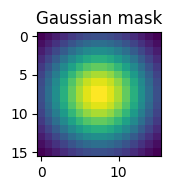
\includegraphics[scale=0.8, max width=\linewidth]{./fig/energy-based-model/predictive-coding/cell012.png}
	\caption{cell012.png}
	\label{cell012.png}
\end{figure}
損失関数を定義する.
\begin{lstlisting}[language=julia]
function calculate_total_error(error, errorh, variable::RaoBallard1999Model, param::RBParameter)
    @unpack r, rh, U, Uh = variable
    @unpack α, αh, σ⁻², σ⁻²td, k₁, λ = param
    recon_error = σ⁻² * sum(error.^2) + σ⁻²td * sum(errorh.^2)
    sparsity_r = α * sum(r.^2) + αh * sum(rh.^2)
    sparsity_U = λ * (sum(U.^2) + sum(Uh.^2))
    return recon_error + sparsity_r + sparsity_U
end;
\end{lstlisting}
シミュレーションを実行する関数を定義する.外側の\jl{for loop}では画像パッチの作成と\jl{r}の初期化を行う.内側の\jl{for loop}では\jl{r}が収束するまで更新を行い,収束したときに重み行列\jl{Phi}を更新する.
\begin{lstlisting}[language=julia]
function run_simulation(imgs, num_iter, nt_max, eps)
    # Define model
    model = RaoBallard1999Model{Float32}()
    
    # Simulation constants
    H, W, num_images = size(imgs)
    input_scale = 40 # scale factor of inputs
    gmask = gaussian_2d() # Gaussian mask
    errorarr = zeros(num_iter) # Vector to save errors    
    
    # Run simulation
    @showprogress "Computing..." for iter in 1:num_iter
        # Get images randomly
        idx = rand(1:num_images)
        img = imgs[:, :, idx]

        # Get the coordinates of the upper left corner of clopping image randomly.
        beginx = rand(1:W-27)
        beginy = rand(1:H-17)
        img_clopped = img[beginy:beginy+15, beginx:beginx+25]

        # Clop three patches
        inputs = stack([(gmask .* img_clopped[:, 1+i*5:i*5+16])[:] for i = 0:2])'
        inputs = (inputs .- mean(inputs)) .* input_scale

        # Reset states
        model.r = inputs * model.U 
        model.rh = model.Uh' * model.r[:]

        # Input an image patch until latent variables are converged 
        for i in 1:nt_max
            # Update r and rh without update weights 
            error, errorh, dr, drh = update!(model, model.param, inputs, false)

            # Compute norm of r and rh
            dr_norm = sqrt(sum(dr.^2))
            drh_norm = sqrt(sum(drh.^2))

            # Check convergence of r and rh, then update weights
            if dr_norm < eps && drh_norm < eps
                error, errorh, dr, drh = update!(model, model.param, inputs, true)
                errorarr[iter] = calculate_total_error(error, errorh, model, model.param) # Append errors
                break
            end

            # If failure to convergence, break and print error
            if i >= nt_max-2
                println("Error at patch:", iter)
                println(dr_norm, drh_norm)
                break
            end
        end


        # Decay learning rate         
        if iter % 40 == 39
            model.k₂ /= 1.015
        end

        # Print moving average error
        if iter % 1000 == 0
            moving_average_error = mean(errorarr[iter-999:iter])
            println("[", iter, "/", num_iter, "] Moving average error:", moving_average_error)
        end
    end
    return model, errorarr
end
\end{lstlisting}
シミュレーションの実行をする
\begin{lstlisting}[language=julia]
# Simulation constants
num_iter = 5000 # number of iterations
nt_max = 1000 # Maximum number of simulation time
eps = 1e-3 # small value which determines convergence

model, errorarr = run_simulation(imgs, num_iter, nt_max, eps);
\end{lstlisting}
\subsubsection{訓練中の損失の描画}
訓練中の損失の変化を描画してみよう.損失が低下し,学習が進行したことが分かる.
\begin{lstlisting}[language=julia]
function moving_average(x, n=100)
    ret = cumsum(x)
    ret[n:end] = ret[n:end] - ret[1:end-n+1]
    return ret[n - 1:end] / n
end

# Plot error
moving_average_error = moving_average(errorarr)
figure(figsize=(4, 2))
ylabel("Moving error")
xlabel("Iterations")
plot(1:size(moving_average_error)[1], moving_average_error)
tight_layout()
\end{lstlisting}
\begin{figure}[ht]
	\centering
	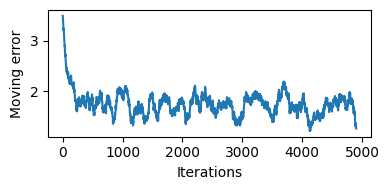
\includegraphics[scale=0.8, max width=\linewidth]{./fig/energy-based-model/predictive-coding/cell020.png}
	\caption{cell020.png}
	\label{cell020.png}
\end{figure}
\subsubsection{重み行列 (受容野)の描画}
学習後の重み行列 ($\mathbf{U}$)を可視化してみよう.
\begin{lstlisting}[language=julia]
# Plot Receptive fields
figure(figsize=(6, 3))
subplots_adjust(hspace=0.1, wspace=0.1)
for i in 1:32
    subplot(4, 8, i)
    imshow(reshape(model.U[:, i], (16, 16)), cmap="gray")
    axis("off")
end
suptitle("Receptive fields of level 1", fontsize=14)
subplots_adjust(top=0.9)
\end{lstlisting}
\begin{figure}[ht]
	\centering
	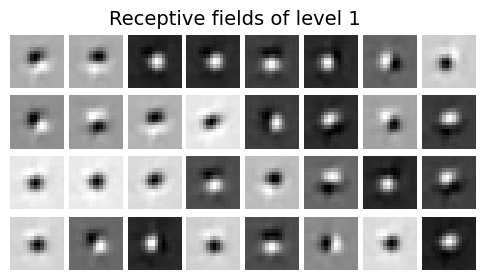
\includegraphics[scale=0.8, max width=\linewidth]{./fig/energy-based-model/predictive-coding/cell022.png}
	\caption{cell022.png}
	\label{cell022.png}
\end{figure}
白色が\textbf{ON領域}\index{ONりょういき@ON領域}(興奮),黒色が\textbf{OFF領域}\index{OFFりょういき@OFF領域}(抑制)を表す.Gaborフィルタ様の局所受容野が得られている.次に,Level2のニューロンの受容野は$\mathbf{U}$と$\mathbf{U}^h$の積を計算することで描画できる.
\begin{lstlisting}[language=julia]
# Plot Receptive fields of level 2
zero_padding = zeros(80, 32)
U0 = [model.U; zero_padding; zero_padding]
U1 = [zero_padding; model.U; zero_padding]
U2 = [zero_padding; zero_padding; model.U]
U_ = [U0 U1 U2]
Uh_ = U_ * model.Uh 

figure(figsize=(7, 3))
subplots_adjust(hspace=0.1, wspace=0.1)
for i in 1:24
    subplot(4, 6, i)
    imshow(reshape(Uh_[:, i], (16, 26)), cmap="gray")
    axis("off")
end

suptitle("Receptive fields of level 2", fontsize=14)
subplots_adjust(top=0.9)
\end{lstlisting}
\begin{figure}[ht]
	\centering
	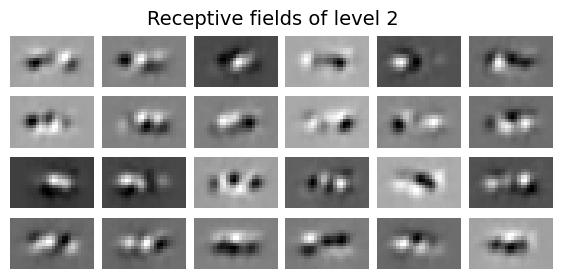
\includegraphics[scale=0.8, max width=\linewidth]{./fig/energy-based-model/predictive-coding/cell024.png}
	\caption{cell024.png}
	\label{cell024.png}
\end{figure}
